\section{Energy budget estimation}
\subsection{UHECRs emissivity}
With the calculated emissivity for the different groups, and the discussion on acceleration there is now the possibility to look from an energy budget viewpoint into the possibility of AGNs being the origin of UHECRs. 
By ignoring the method of acceleration, but considering that our sources must produce the required emissivity one can make a crude estimation of source candidates. 

From the calculation in \ref{sec:emmisivity} the emissivity of UHECRs is given as $1.73 \cdot 10^{44}\rm erg/\rm Mpc^3\rm /yr$ this was calculated from the observed flux of UHECRs from the Pierre Auger observatory \cite{thepierreaugercollaboration2017pierre}.
In this calculation, one needed to confine the area in which these sources could be produced to take into account the energy losses these particles experience. The same argument must be used 
for our emitting sources and therefore one must use the emissivity of our sources at a redshift very close to Earth. To get a comparable emissivity one evaluates therefore the emissivity at redshift $z=0.01$. The result is shown in figure \ref*{fig:flux_UHECRs}

\begin{figure}[H]
    \centering
    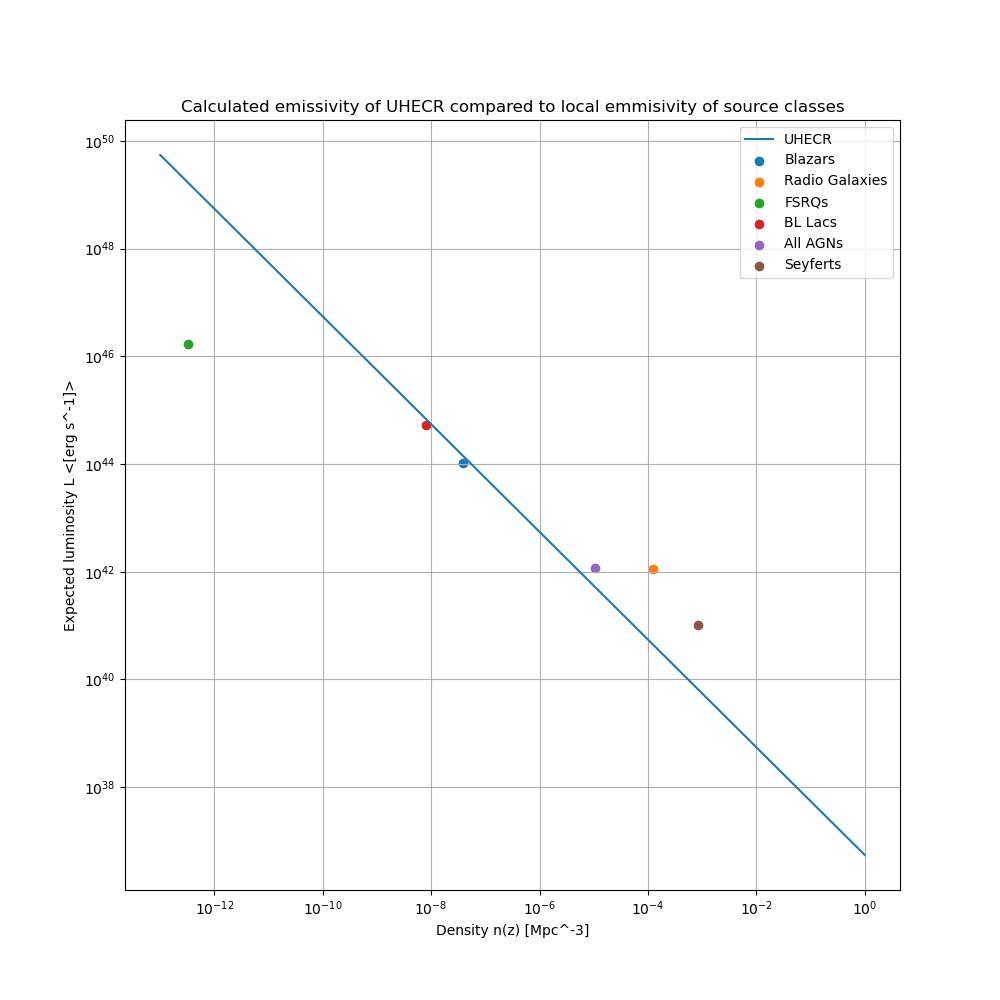
\includegraphics[width = 0.7\textwidth]{new_plots/L_n_uhecr_calc.png}
    \caption{UHECR emissivity for the four different classes of AGNs.}
    \label{fig:UHECR}
\end{figure}

This figure shows that most classes of AGN produce a total emissivity in X-ray comparable to the one energy detected by the Pierre Auger observatory. The only exception is the FSRQs which are not numerous enough at this redshift. 
To criticize this very crude estimate, one must first note that the correlation between X-ray luminosity and UHECR luminosity is not well-defined and should include parameters that are not accounted for.
In addition to this one has not done any separation between jet-dominated and non-jet-dominated AGNs, and even though our non-jet-dominated AGNs are capable of producing the required x-ray luminosity
the mechanism of transferring this energy into UHECRs as talked about in section \ref{sec:Expt_lum} is not well understood. 

%A very interesting point is that the only candidate not able to produce the required emissivity, the FSRQs, are the ones where according to \cite{Wei-Hao_2003} one could find a Kerr black hole. 
%A Kerr black hole is needed in mechanisms such as the Blandford-Znajek mechanics which is a possible way of accelerating and beaming particles into jets. One notes that it is not only that mechanism that could accelerate UHECRs and 
%the outflows discussed in \cite{Laha_2021} would have an acceleration mechanism as well. The author of this paper notes that the energy gain in these outflows is not known and therefore one cannot say if they are powerful enough to produce extra galactic UHECRs. 

Nevertheless, the result does not rule out the possibility of AGNs being the origin of the UHECR diffuse flux. 


\subsection{Neutrino emissivity}
Similarly, for the UHECRs, we calculated the local emissivity for the neutrinos in section \ref{sec:emmisivity}. The result was $1.2 \cdot 10^{44} \rm erg/\rm Mpc^3\rm /yr$ which is a factor similar to that of UHECRs.
In the calculation, the diffuse neutrino flux on Earth was taken from the IceCube observatory \cite{Abbasi_2022} and the energy range was taken to be $1\rm TeV - 10\rm PeV$ corresponding to the astrophysical neutrino flux.
The difference between the UHECR flux to the neutrino flux is the energy loss mechanism. The effect of a very limited energy loss mechanism means that the emitting area is now the whole universe. To reach a comparable emissivity one must therefore take a redshift-dependent average of the sources over the whole universe.
One does this by scaling the emissivity at redshift $z$ with the corresponding energy loss for a neutrino from that redshift given as $(1+z)$ and then taking the average emissivity to get a comparable emissivity.
The resulting figure is shown in figure \ref{fig:neutrino}.

\begin{figure}[H]
    \centering
    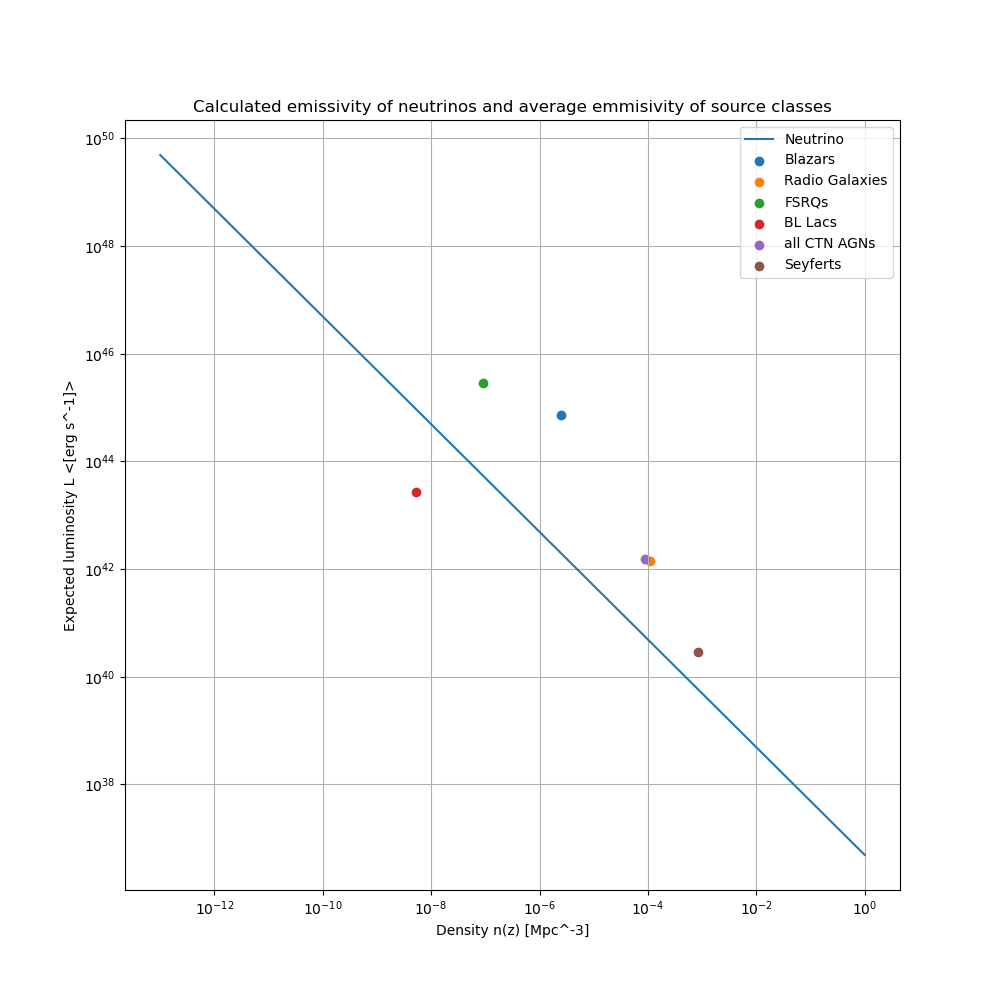
\includegraphics[width = 0.7\textwidth]{new_plots/L_n_neut_calc.png}
    \caption{Neutrino emissivity for the four different classes of AGNs.}
    \label{fig:neutrino}
\end{figure}

This figure shows that the neutrino flux can be produced by all classes except 
the BL Lacs. This is an effect of the averaging since the BL lacs have a negative evolution.
The opposite is the FSRQs which now can produce the required emissivity.

In addition to the average picture given in figure \ref*{fig:neutrino} one can also calculate the diffuse neutrino flux directly from the different classes of AGNs. This is done by modifying the transfer function defined in \cite{Palladino_2020} and this is given as


\begin{equation}
    \frac{d\phi_\nu}{dE_\nu} = \int_0^{z_{max}} \frac{D_H}{E(z)} \frac{L(E_\nu (1+z),<L_x>(z))}{(1+z)^2} \rho(z) dz
\end{equation}

Here $D_H$ is the Hubble distance, $E(z)$ is the function defined in section \ref{sec:comoving_distance}, $L(E_\nu (1+z), <L_x>(z))$ is a power law representing the neutrino flux at the source, which when integrated reproduces the average source luminosity at redshift $z$, and $\rho(z)$ is the number density of the sources at redshift $z$.
With this function, we can calculate the expected diffuse flux of neutrinos from the sources. The difference between \cite{Palladino_2020} and I, is the inclusion of a luminosity dependence in the power-law function. This is done to account for the different average luminosity of the different classes of AGNs which was assumed constant in \cite{Palladino_2020}. 
The assumption of a constant luminosity is not a bad one since the luminosity of the different classes is not changing significantly over the redshift range, but it is still a simplification, especially for the Blazar class. The form of the spectra is taken to be identical to the observed neutrino flux by ICE CUBE which is defined in section \ref*{sec:emmisivity_neutrinos}.
The result is shown in figure \ref{fig:neutrino_diffuse}.
\begin{figure}[H]
    \centering
    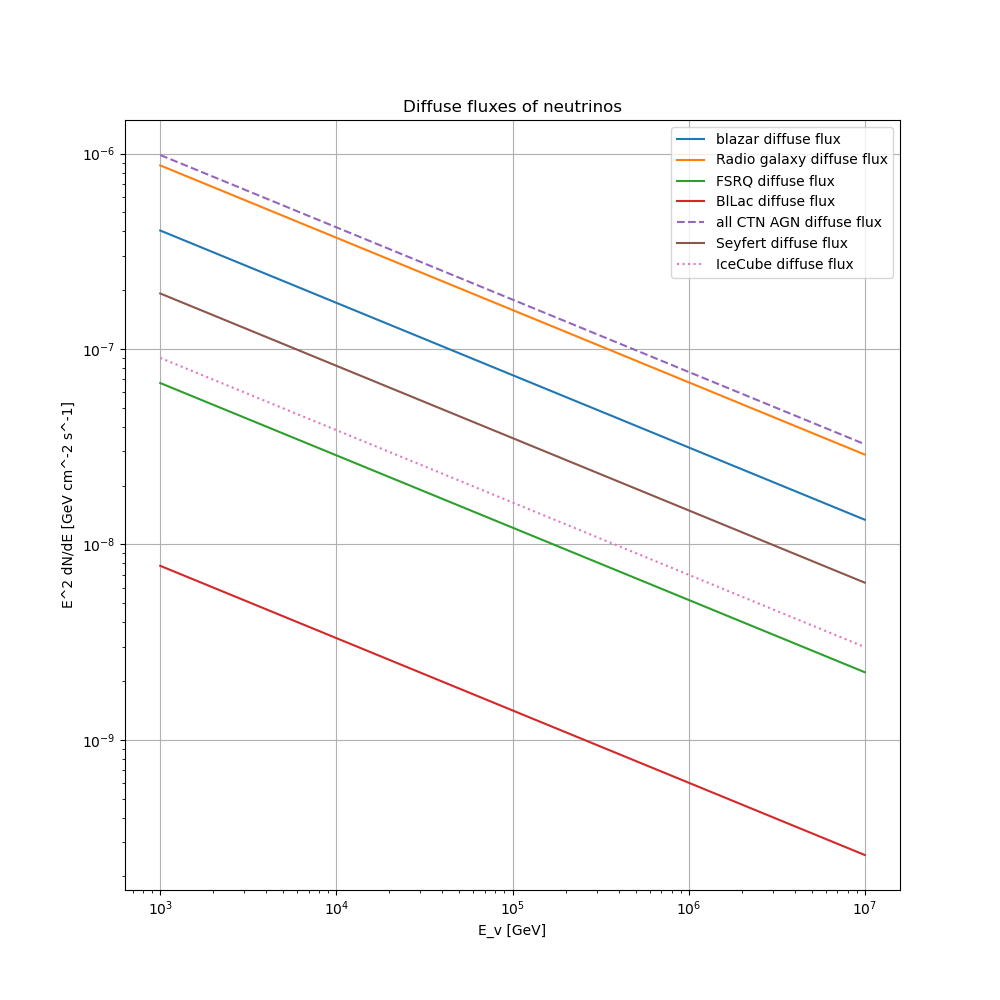
\includegraphics[width = 0.7\textwidth]{new_plots/diffuse_fluxes_neutrino_no_cutoff.png}
    \caption{Diffuse neutrino flux for the four different classes of AGNs.}
    \label{fig:neutrino_diffuse}
\end{figure}

What one sees here is almost the same result as the crude average which is good. The FSRQs and Bl lacs are now not able to produce the diffuse flux but the rest are. 
The fact that all sources are overshooting the observed neutrino flux would be a problem if we had a more constrained solution. Any model that overshoots could not be the source since it is not what we observe, but in our case, 
our solution rests on the fact that the neutrino luminosity is equal to the x-ray, an assumption easily broken and without nuance. Therefore, the only concrete conclusion one can draw from this is that the neutrino flux can be produced by the AGNs since they can produce the required emissivity.
Several papers such as \cite{Kurahashi_2022} talk about the lack of any anisotropy in the observed diffuse neutrino flux. Such an anisotropy would introduce a required density of sources. This would be a problem for the more obscure sources such as FSRQs and could further limit our predictions.

This result in figure \ref*{fig:flux_neutrinos} is obtained differently than in figure \ref*{fig:neutrino} and therefore the agreement between them is a good sign. The argument that the x-ray luminosity should have the same value as the neutrino luminosity is not a bad first guess, but it does leave a lot to be desired. 
This flux model does not incorporate any parameters of the AGN other than emitting strength, and therefore it is not a very nuanced model. A first fix could be a model that includes the jet orientation and most importantly the acceleration mechanism one could imagine happening. What this 
crude model can show is that these objects do produce enough power. To make the estimation better without doing much more work, one could look at the gamma-ray luminosity functions of the same sources and see if they can produce the required neutrino flux. Gamma-ray production is a natural consequence if one is using the pion decay model
for neutrino production. In this way, one could more easily constrain the neutrino production with the gamma-ray production. 
This is however outside the scope of this paper and will be left for future work. 

%\subsubsection{AGN as the origin of the astrophysical particles}
%Both the diffuse flux of neutrinos and UHECRs estimate an emissivity that is comparable to the x-ray emissivity of our sources. The correlation between x-ray luminosity and the production of these ultra-high energy 
%particles is also not unfounded since both require a high number of charged particles. For these arguments, one could imagine that AGNs of all classes can produce these particles. 

